%% ================================================================================
\chapter{Theory}
\label{ch:theory}
%% ================================================================================
%The theory chapter. These are references \cite{aPaper}, \cite{aThesis}, \cite{aWiki}. Figure \ref{fig:dummy} shows a placeholder. 
%
%\begin{figure}
%  \centering
%  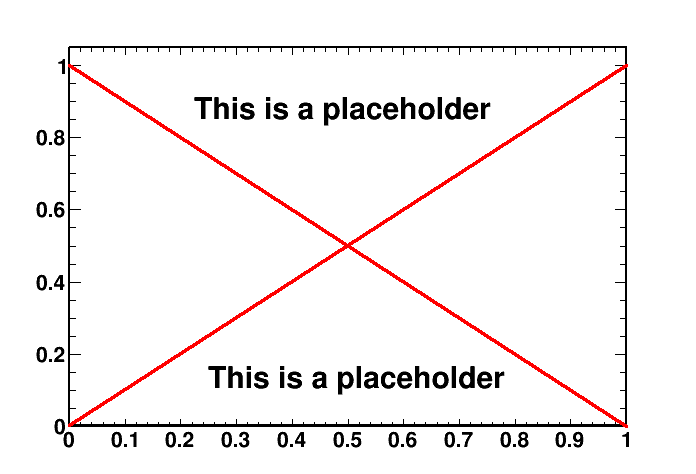
\includegraphics[width=.9\linewidth]{pic/dummy.png}
%  \caption{This is a dummy plot.}
%  \label{fig:dummy}
%\end{figure}
%
%\section{A section}
%\label{sec:section}
%Here we have Section \ref{sec:section}. \todo{This is a TODO marker} You might need this.

\section{Our Milky Way}

\subsection{General properties}


\begin{figure}[h]
  \centering
  \begin{minipage}[h]{0.45\textwidth}
  	\centering
	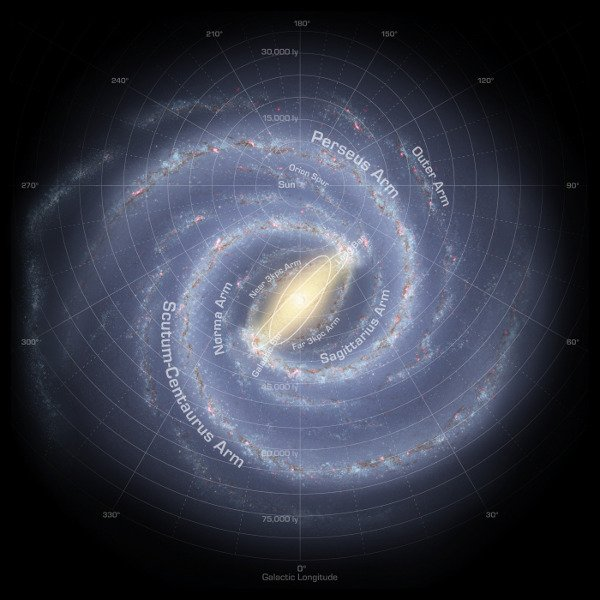
\includegraphics[width=1.\linewidth]{pic/theory/top_galaxy_map.jpg}
  	\subcaption{source: http://galaxymap.org/drupal/node/171}
  	\label{fig:top_gal_map}
  \end{minipage}
  \hfill
  \begin{minipage}[h]{0.45\textwidth}
	  \centering
	  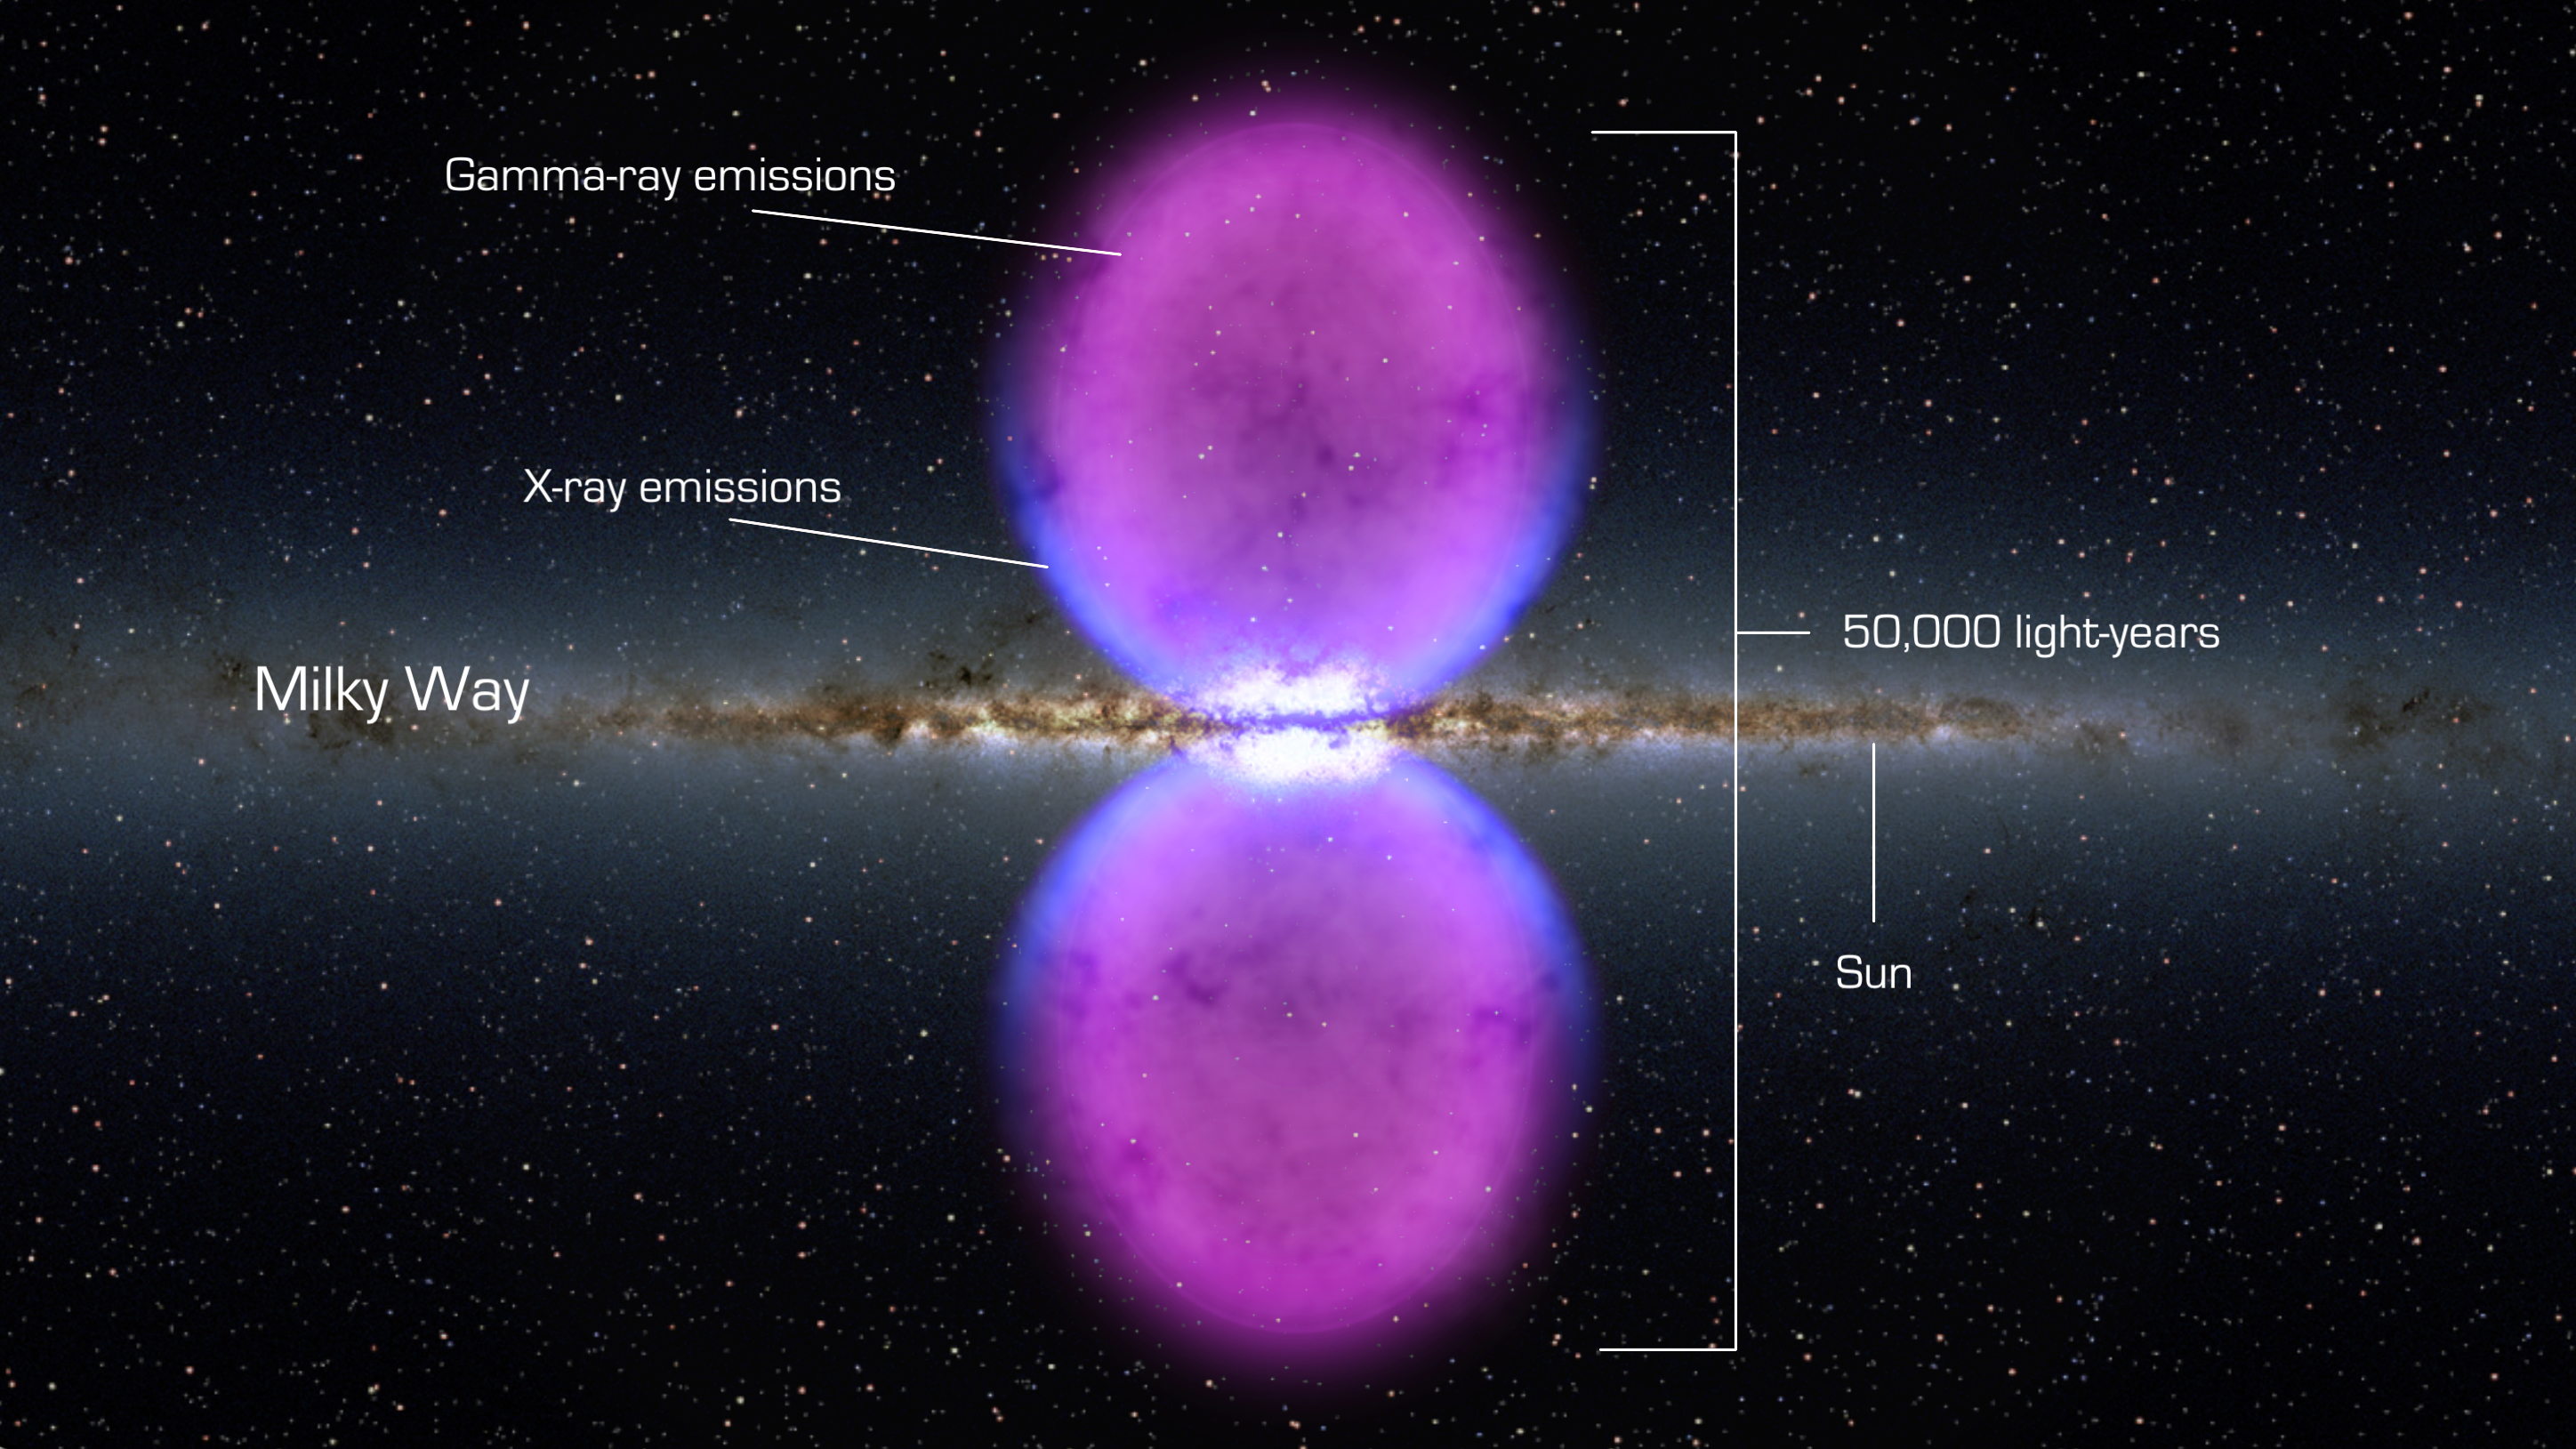
\includegraphics[width=1.\linewidth]{pic/theory/Fermi_bubble.jpg}
	  \subcaption{source: NASA's Goddard Space Flight Center}
	  \label{fig:fermi_bubbles}
  \end{minipage}
  \caption{The Milky Way, as seen from two different angles.}
  \label{fig:Galaxy_maps} 
\end{figure}

For a long time, people thought the universe was constituted of only one galaxy, the Milky Way, the one in which the Sun and the Earth orbit. The discoveries of other galaxies in the universe came only in the 20's thanks to Edwin Hubble. There is still a lot of unknown  around those objects, but the Milky way is pretty well known and will play a major role in the following chapters. Its shape, density and composition are three main factors playing a role in cosmic ray physics and can not be avoided.

First of all, the Milky Way is a barred spiral arm galaxy, meaning it has two main spiral arms, connected in their center by a straight galactic bar. Those arms and bar have higher matter concentration than the rest due to the way stars orbit around the center. Its diameter exceeds 40 kpc for a mass of around $10^{12} M_\odot$ and a thickness under 1 kpc. The Sun and the Earth are rotating 8 kpc from its center in 240 Myr.
All the different objects of the galaxy can be found in this thin disk of matter, mainly in the spiral arms. It includes the stars, planets and over massive objects, but also all the dust and gas clouds. As seen from the Earth, the disk looks like a narrow band of a few degrees in latitude, but with a very high concentration of gas and dust.
In 2010, two large scale structures were detected to the north and the south of the GC. With a diameter of 7kpc, these two "bubbles" extend up to 40 degrees in latitude and 20 in longitude. They are a source of high energy gamma-rays and were detected by the Fermi Large Area Telescope (LAT).

The disk of the Milky way is composed of matter in different forms, like stars, gas or dust. Stars are one of the first source of the interstellar radiation field (ISRF). They can be compared to black body radiating at different energies depending on their temperature. They are the main source of UV photons, that play a major role in the gas evolution. Stars are forming inside gas and dust clouds, collapsing on themselves under their own gravitational pressure.
The gas is composed in the vast majority of hydrogen, but heavier elements and even molecules can be found at the center of large clouds where ultra-violet light can not penetrate. One of these is the CO molecule, often used to as a tracer of molecular clouds. Even if molecules can only be found where the UV starlight can not break them apart, molecular clouds (MC) will designate large region of gas and dust, that can possibly contain stars inside.
\todo{add gas/dust ratio} Dust is also present in the galactic disk. It can be warmed by the starlight, and cooled via infrared light emission. This IR source is also part of the ISRF.

Electromagnetic field runs all across the milky way, taking its source in rotating stars, molecular clouds, or any moving charged particle. It has been observed and measured, but it is very complex and has no favourite direction at small scales (interstellar scale).

\subsection{Dark Matter}

\begin{figure}[h]
 \centering
 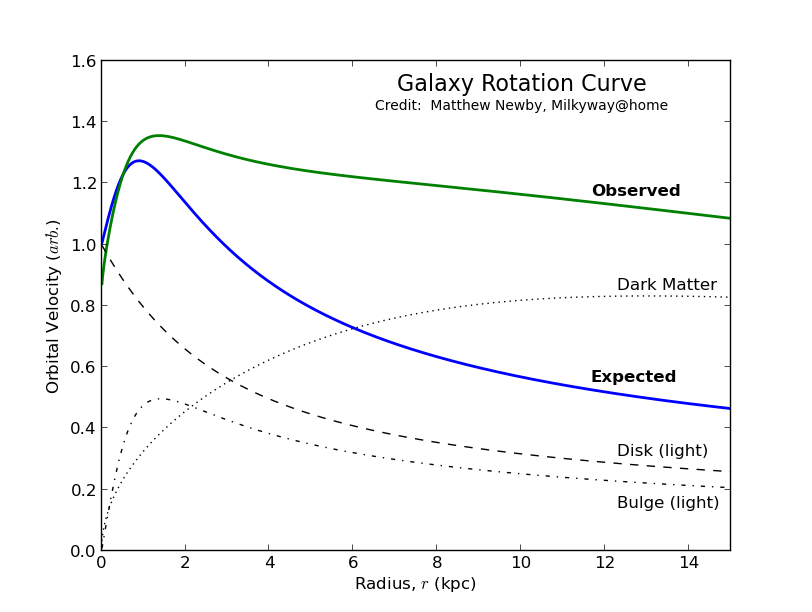
\includegraphics[width=.5\linewidth]{pic/theory/gal_rotation_curve.png}
 \caption{Orbital velocity of the Milky Way as a function of the radius. A clear discrepancy between the theory and the observation can be seen above a 2 kpc radius. Source: Matthew Newby, Milkyway@home}
 \label{fig:gal_rotation_curve}
\end{figure}


The shape of spiral galaxies is well known today, with thousands of examples throughout the universe. This knowledge can be used to mathematically simulate them, and in particular their rotation speed as a function of the distance to the center. It was a big surprise when the observed angular speed did not match the theory. One of the solution to explain this difference was the introduction in the standard model of dark matter (DM), which was suppose to bring a lot of invisible mass into the system. It still has not been observed and a few theories exist on its exact nature. But even without knowing exactly what it is, its mass distribution can still be deduced from the observed rotation curve of the galaxy. The predicted distribution is a spherical halo extending way beyond the 40 kpc of the galactic matter disk. It's density peaks in the GC, and decrease with the radius following a particular density profile. The exact profile is not known, but a popular one is the Navarro-Frenk-White (NFW) profile defined as follows :

\begin{equation}
\rho (r) \propto \frac{1}{\left( r/r_S \right) \left( 1 + r/r_S \right)^2 }
\end{equation}

where $r_S$ is the scale radius.

One of the most popular is the Weakly Interacting Massive Particles (WIMP). They are supposed to be non standard particles with a large mass, neutral, and only sensitive to the weak force, making them very difficult to observe. But no particles of the standard model has the right properties. 


\section{Tools}
%Energy spectra
%Intensity, Flux

To speak about cosmic-rays, one often speaks about their spectral shape, or energy spectrum. These terms refer to the particle flux ($\Phi$ in $GeV^-1.s^-1.cm^-2.sr^-1$) as a function of their energy (in $GeV$).  In other terms, how many particles of a given energy would a one centimeter square instrument observe in one second. This can often be modeled by a power law of the form $\Phi \propto E^{-\alpha}$  where $\alpha$ is called the spectral index. If $\alpha$ is small, the spectrum is said to be "hard", because there are an important proportion of high energetic particles. On the contrary, a "soft" spectrum has a bigger spectral index and describe a lower density of high energy particles compared to low energies.

In the following chapter though, the preferred representation of the energy distribution is via the energy flux (in $GeV.s^-1.m^-2.sr^-1$), simply obtained by multiplying the particle flux by its energy square ($E^2 \times \Phi(E)$). In other terms, how much energy does the instrument receive every second for particles of a given energy E. This is only done to facilitate the reading of the graphs and does not affect the underlying physics.

The terms of "soft" and "hard" can be applied to any kind of energy spectrum, even if it is not a power law, it will only describe the relative proportion of high and low energy particles.




\section{Physic of cosmic rays}

\subsection{Creation of CR}
\label{sec:creation_of_CRs}
%		-supernovae (SNR)
%		-AGN (activ galactic nuclei)
%		-pulsars, quasars

Several sources of cosmic rays exist in the universe. Cosmic rays are very energetic and thus can only be produced by very energetic phenomena. Particularly powerful events are supernovae, ejecting relativistic particles during the burst. The dying star will eject a lot of its mass to form a supernova remnant (SNR) surrounding either a white dwarf, a neutron star or a black hole depending on the initial mass of the star. These SNR could also play a role after the explosion via the Fermi process. An already energetic particle would bounce in the shock wave created by the explosion, and gain energy via hydrodynamic or magneto-hydrodynamic before escaping when the energy is sufficient.
An other important source of cosmic rays are the pulsars. These rapidly rotating neutron stars and their intense electromagnetic field create high energy particles such as protons and electrons. This can last as long as the pulsar rotates fast enough, but it can takes 10 to 100 Myrs before the turn-off occurs.
A third source are the actives galactic nuclei (AGN), also known as quasars. These objects consist of a super-massive black hole at the center of a galaxy. First discovered thanks to their radio emission, they are also able to eject CR, certainly via Fermi or centrifugal acceleration.


\subsection{Propagation of CR}
%Propagation through the galaxy
%	-random B field -> no way to backtrace a CR
%	-interaction, shocks in MC
%	-Diffusion coefficient
%		-Can be different in disk, bubbles, or outside
%	-different diffuse coef mean different densities
%		-in MC, bubbles, outside
%		-can observe this inhomogeiniies via gamma rays

Once they are emitted, the cosmic rays propagate through the galaxy under the influence of different interactions.
The first one to notice is the complex magnetic field created by all sorts of objects, from stars to molecular clouds or any distribution of charged particles. It is not particularly strong \todo{put values} compared to the heliosphere or what can be created on Earth, but its very large scale suffice to bend the CR's path in all direction until the point where it is impossible to backtrack their origin.
An other possible interaction is the collisions with other particles. It will obviously depends on the density distribution of those colliders in the galaxy. We can expect a higher number of those in the disk, where the density of molecular clouds is the highest.

All these influences can be modelled by a diffusion model, mainly defined by its diffusion coefficient D, which describes the average distance travelled by the particles during a certain time. The higher the coefficient, the faster a particle will diffuse in the galaxy. Each phenomenon can be attributed one of those coefficient to describe its effect on the cosmic rays. \todo{give values for Dmag, Dcoll...}
While the diffusion coefficient for the galactic magnetic field can be taken as constant throughout the milky way, the diffusion coefficient due to collision is proportional to the particles density. We can then expect a smaller coefficient in molecular clouds, where the density can reach \todo{value!}.

This coefficient will also define the cosmic ray densities in various locations of the galaxy. Indeed, the more a particle's path is twisted and convoluted, the harder it will be to move away from its origin. This way, a higher density of cosmic rays can be found in low diffusion coefficient areas like molecular clouds. In comparison, the region outside the galactic disk has a low density of CR due to a weak electromagnetic field and small gas and dust density. However, the bubble region is outside the disk and has a higher concentration of CR than other regions outside the disk. This is due to a direct outward emission of CR from the GC region. With a high diffusion coefficient, these CR are ejected light years away (see Fig. \ref{fig:fermi_bubbles}), forming two symmetric regions extending north and south up to 40 degrees in latitude.

The consequences of such diffusion processes is an isotropic cosmic-ray sky on Earth. In whatever direction the instruments look at, they measure the same CR flux. This complicate a lot their study, since no information about their origin or their journey can be learned from direct observation. 
%It is where gamma-rays enter the scene to play a major role in the indirect detection methods.

\subsection{CR as observed from Earth}

\begin{figure}[h]
 \centering
 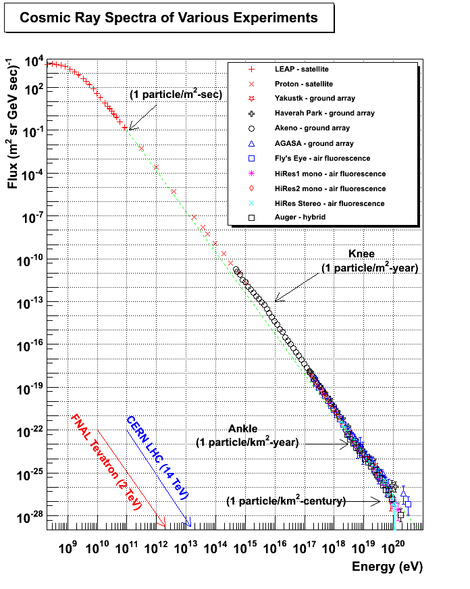
\includegraphics[width=.5\linewidth]{pic/theory/CR_spectrum.png}
 \caption{Cosmic ray spectrum as seen by several experiments. The "leg" can be seen with a "knee" around $5.10^{15} eV$ and two different spectral indices on both sides. Two of the best human attempts to recreat very high energetic particles are shown and give an idea how powerful CR can be.
 Source: http://www.physics.utah.edu/~whanlon/spectrum.html}
 \label{fig:CR_spectrum}
\end{figure}

The one and only CR spectrum that can be obtain from observations on Earth is shown on Figure \ref{fig:CR_spectrum}. It is the same in every direction as far as the measurement uncertainties can tell. The isotropic arrival direction of CR is measured with great care and any anisotropy, if existing, is below the instrument precision.
The CR spectrum is composed of three main features that form a "leg". The "knee" around $10^{7} GeV$ marks the separation between two different power laws in $E^{-\alpha}$. A slightly harder one below that is thought to be composed of galactic CRs, and a softer one above that is supposed to be of extra-galactic origin. The spectral index does not change much, from 2.7 below to 3 above, due to different production mechanism.
As indicated on Figure \ref{fig:CR_spectrum}, the corresponding flux of particle is very low and statistical fluctuations are not negligible at high energies. Especially at the "ankle", above $10^9 GeV$, where only very few particles were detected.


\subsection{Gamma-ray creation}
%		-pion decay
%		-bremmstrahlung
%		-inverse compton

Since the cosmic rays we observe on Earth can not give us a clue about their origin, some indirect detection methods are required. Luckily, cosmic rays interact in a lot of ways with their environment, as described in the previous section. These interactions can leave detectable traces that can be observed. The most common is the production of light, via creation of high energy photon in the GeV range. Once created, these gamma rays can be blocked or absorbed, but not deflected. Linking the gamma-ray and cosmic ray requires to know the processes in play. Here is a list of the main phenomena.

\subsubsection{Pion decay}
%Explain phenomenon
%Explain expected gamma ray spectrum, propagated proton distribution.

%The high energy protons can produce $\pi^{0}$ which decay almost immediately in 2 gammas of equal energy.

The hadronic cosmic rays  particles interact with the interstellar medium and can lead to pion $\pi^0$ production. Any CR nuclei can result in pion production, but since protons are the most abundant particles, they will dominate the production. 
These newly created pion can rapidly decay into a pair of gamma-rays (99\% of the time) or e+e- pair (negligible).




\subsubsection{Bremsstrahlung}
%Explain phenomenon
%Explain expected gamma ray spectrum


The charged CR passing near an other charged particle of the ISM or in a magnetic field will be deflected by the electromagnetic interaction. In the process, the CR will lose energy via the emission of photons. The energy of the latter will depend on the energy of the electron and the intensity of the electromagnetic field. The more the electron is deflected, the higher the energy of the emitted photons.
Even though proton CR are charged, the main source of bremsstrahlung gamma-rays is electrons and positrons. This is due to the much lower mass of the electrons, making them easier to deflect.

\todo{give numbers for B field and proton in MC}


\subsubsection{Inverse Compton}
%Explain phenomenon
%Explain expected gamma ray spectrum


A third process can take create gamma-rays when the CR electrons interact with a photon of the interstellar radiation field (ISRF). When a high energy electron collides with a low energy photon, the electron can transfer some of its kinetic energy to the photon, giving him enough energy to enter the gamma range.

So number of gamma rays coming from inverse Compton is directly linked to the electron distribution and the ISRF of the galaxy. The latter is composed of three major components, the starlight, the dust emission and the cosmological microwave background (CMB). The first component is directly linked to the star distribution, and will be dominant in the disk, where all the star are concentrated. The starlight emits as a black body, peaking in the UV range. The dust emission comes from the infra-red emission of warm dust. It will also be mainly present in the disk, since the dust clouds are pretty flat. Finally, the CMB is peaking in the microwave range but is uniformly present everywhere in the universe, and therefore in the galaxy. It will be dominant where the two others are negligible, namely outside the galactic disk.


\todo{talk about synchrotron and ionization losses}

\subsubsection{Other sources}
%Gamma-ray burst
%Pulsars

The three previously described processes are general processes that can happen everywhere at any energy. But even though the process might always be the same, two class of sources can be defined: the diffuse and the point sources. 
The first correspond to all the CR propagating through the ISM and interacting with its components. It will be the object of study of the following chapters. 
The second are the gamma-rays produced directly at the CR origin (in SNR, AGN or pulsars as described in section \ref{sec:creation_of_CRs}). Every one of these event should be studied separately and are still not understood perfectly. Since these sources are very far away and can not be resolved by the instruments, they will be referred to as point sources in the following chapters. The spectral shape of these events is generally known and categorized as a function of the event type. This makes the recognition easier and both emissions can be separated 
this way.


%Other sources of gamma-rays exist in the universe that will complicate the observations. Gamma-rays are very energetic and thus can only be produced by very energetic phenomena. The gamma-ray bursts for example were discovered in the late 60's when U.S. satellites were build to detect nuclear weapon tests. These two events produce gamma-rays, but the first one is much more powerful, sometimes emitting more energy than the Sun will in its entire life-time. It is thought to be emitted by supernovae in distant galaxies or the merging of two neutron stars. These events are short (from milliseconds to hours) and will not be dominating the observations.
%An other source is the pulsar gamma-ray emission, and even though they are less energetic, their long-term production make them one of the first sources of observed gamma-rays. It can be said the same about quasars or active galactic nuclei (AGN).
%All these sources produce high energetic cosmic-rays that will lose energy via the different processes described earlier, and produce gamma-rays. 


\subsection{Gamma-ray observations}

Gamma-rays are not easy to observe from Earth, simply because they are absorbed by the atmosphere. It is a chance for life to develop, but complicates their observation. To measure them, the instrument has to be launched in orbit above the atmosphere, where gamma-rays are not yet absorbed. For example the Fermi Large Area Telescope (LAT) mounted on the ISS do the job with a lot of success. This instrument maps the gamma ray sky between 20 MeV and 300 GeV \todo{cite}, detecting all the point sources emission, but also the diffuse background emission.


%The diffuse cosmic ray emission that we are interested in can be obtained after modeling and subtracting the contribution of the over sources. This allows us to compare the observation with the models we obtain from the previous three interactions.


In theory, the knowledge of the processes that generate gamma-rays from cosmic-rays and the precise composition of the Milky Way should allow to explain the observations. Propagation models and simulations are able to output the expected energy spectrum of gamma-rays reaching Earth from an initial distribution of cosmic-rays (not taking the point sources into account). But some problems show up when confronting the theory and the observations, as will be discussed in the following section.



\section{What are the unresolved problems of the precedent chapter}
%What are the unresolved problems of the precedent sections:
%	-Bad fits in bubbles and disk	
%	-Spherical gamma-ray excess in GC when fitting spatial templates
%		-DM studies
%			-Hooper
%			-others...
%		-MSP studies
%			-Fermi
%			-Hooper
%			-Weniger
%	-High energy tail flux too hard
%	
%
\begin{figure}
 \centering
 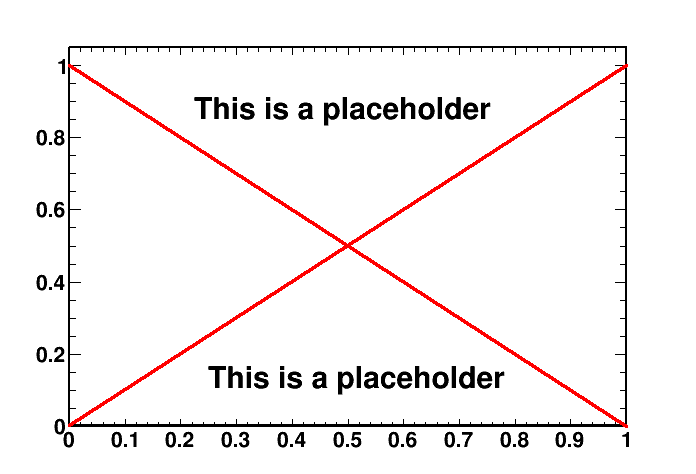
\includegraphics[width=.9\linewidth]{pic/dummy.png}
 \caption{chi2 distribution of first fits (not mines)}
 \label{fig:first_BKGonly_fits}
\end{figure}



\begin{figure}
 \centering
 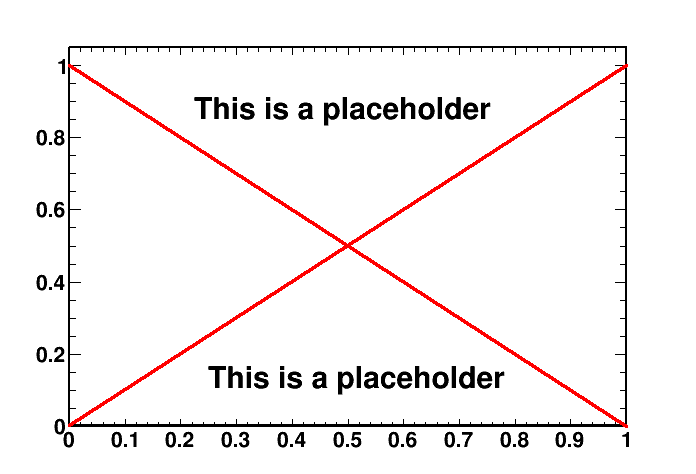
\includegraphics[width=.9\linewidth]{pic/dummy.png}
 \caption{shape of the excess}
 \label{fig:first_BKGonly_fits}
\end{figure}

Several studies have already tried to see how the predictions of the gamma rays emission and the observations compare. The three main phenomena were modelled to try to recreate the spectrum observed here on Earth. The results are clear, they do not always match.
Even though the observations of the poles or any high latitude regions can be well explained by a PCR, BR and IC component, the models have troubles to reproduce the surroundings of the galactic disk, and in particular the GC or the Bubbles. 
Two main problems can be identified. A high energy deficit in the models, where the high energy tail (> 50 GeV) observed can not be reproduced, and a spherical excess centred in the GC around 2 GeV.

The first one shows a lack of high energy cosmic-rays in the models. A mean of injecting more relativistic particles has to be found in order to fill this gap. One explanation could be that we do not observe only diffuse emission in the disk. The point source emission could not be totally subtracted due to the high density of sources. The CR that do not have the time to propagates have a harder spectrum, thus providing a higher ratio of high energy gamma-rays.

Two main ideas have emerged to explain the spherical excess.
First is the presence of dark matter in the galaxy in the form of weakly interacting massive particles (WIMP). The spatial distribution of these particles would follow a Navarro-Frank-White (NFW) profile centred at the GC. They are also expected to produce gamma rays when annihilating with each other via hadrons production. In theory, if the mass of a WIMP particle is around 50 GeV, the expected gamma spectrum would peak around 2 GeV, where the excess is observed. \todo{cite}
The study of the excess could put strong limits on the mass and annihilation cross section of such WIMP and confirm, or infirm the theory.
The second theory does not involve new physic, but unobserved millisecond pulsars. They would also be spherically distributed around the GC and their gamma spectrum peaks around 2 GeV. A few thousands of them would be needed to recreate the intensity of the excess. The main default of this explanation resides in the fact that we have observed only a few hundreds pulsars so far when we expect ten times more.







































